\documentclass[11pt,dvipdfmx]{jarticle} 

% AMS font を使う
\usepackage{ascmac}
\usepackage{amsfonts}
\usepackage{graphicx}
\usepackage{amsmath}
\usepackage{bm}
\usepackage{algpseudocode,algorithm}
\usepackage{theorem}
\usepackage{latexsym}
\usepackage{mathtools}
\usepackage{comment}
\usepackage{color}
\mathtoolsset{showonlyrefs=true}
\def\qed{\hfill $\Box$}
\algrenewcommand{\algorithmicrequire}{\textbf{Input:}}
\algrenewcommand{\algorithmicensure}{\textbf{Output:}}
\DeclareMathOperator*{\argmax}{arg\,max}
\DeclareMathOperator*{\argmin}{arg\,min}
\numberwithin{equation}{section}
\newtheorem{theorem}{定理}[section]
\newtheorem{lem}{補題}[section]
\newtheorem{proof}{証明}
\newtheorem{coro}{系}[section]
\renewcommand{\theproof}{}
% 紙のサイズなど.だいたい A4 むけ.
\oddsidemargin=0cm \evensidemargin=0cm
\topmargin=0cm \headheight=0cm \headsep=1cm
\textwidth=16cm  \textheight=23cm

\begin{document}
\thispagestyle{empty}
\vfill
\hfill 電気通信大学情報理工学部 \\
\hfill 情報・通信工学科情報数理工学コース卒業論文

\vfill
\begin{center}
  \Large Partition制約付き最小化ナップサック問題に対する3-近似アルゴリズム
\end{center}
\vfill
\begin{center}
    平成30年  1月31日
\end{center}
\vfill
\begin{center}
  \large
  情報数理工学コース\\[1cm]
  学籍番号 1411070\\[1cm]
  木村優貴
\end{center}
\begin{center}
  指導教員 村松正和
\end{center}
\vfill

\pagebreak

\section{はじめに}
    離散最適化にはNP困難な問題が多数存在する.
    NP困難な問題に対して用いられるアプローチは3つある.\par
    1つは多項式時間で終了する保証はないが,最適解を導出するアプローチである.
    このアプローチについては切除平面法\cite{kp_np},分枝限定法\cite{kp}などが研究されている.
    しかし,このアプローチの問題点は,NP困難な問題に対する多項式時間アルゴリズムは現在知られていないので,
    問題のサイズによっては現実的な時間内では最適解を求めることができない場合があることである.\par
    もう1つは最適解を求めることを諦め,近似解を現実的な時間で求めるという近似アルゴリズムの設計によるアプローチである(\cite{apx_des},\cite{apx_al}).
    このアプローチには2通りある.
    1つは実行可能な時間内で保証のない近似解を求めるアプローチである.このアプローチについては遺伝的アルゴリズムなどが研究されている.
    もう1つは多項式時間で保証のある近似解を求めるアプローチである.\par
    本稿ではこのアプローチの中でも代表的手法である主双対法について紹介し,これを用いて近似アルゴリズムの設計を行う.\par
    品物をナップサックに容量を超えることなく詰め込む時に,詰め込む品物の価値の総和を最大化することを目的とした問題をナップサック問題と呼ぶ\cite{kp}.
    ナップサック問題はネットワーク構築\cite{kp_ex1}や資源配分問題\cite{kp_ex2}など現実問題に対しても多く用いられている.
    さらに,この問題はNP困難であることが知られている(\cite{kp_np},\cite{np_c}).
    この問題の様々な拡張に対する近似アルゴリズムの研究が広く行われている.\par
    最小化ナップサック問題は,
    品物をナップサックに価値の総和をある需要以上に保ちつつ,詰め込む品物の重さの総和を最小化することを目的とする問題である\cite{apx_des}.
    この問題もNP困難な問題であることが知られており,最適解の導出や近似アルゴリズムの設計が広く行われている.\par
    本研究は,この最小化ナップサック問題に対し新たな制約を加え,拡張した問題に対して制度保証のある近似アルゴリズムの提案を行う.
    本稿の2章では近似アルゴリズム,最小化ナップサック問題などの事前知識について説明し,
    3章と4章では最小化ナップサック問題に対し,品物の集合に関する制約を加えた問題に対する近似アルゴリズムについて記す.
    また,本稿の末尾にはそれぞれの近似アルゴリズムの詳細を示した疑似コードを添付する.

\newpage
\section{事前知識}
    \subsection{近似アルゴリズム}
        近似アルゴリズムとは,最適値に十分に近い目的関数値が得られるような解を求めるアルゴリズムである.
        近似アルゴリズムの中でも最適化問題の全ての入力に対して最適値の$\alpha$倍以内の値を持つ解を返すアルゴリズムを
        その最適化問題に対する$\alpha$-近似アルゴリズムと呼ぶ\cite{apx_des}.この時の$\alpha$を近似率と呼ぶ.
        最小化問題に対しては$\alpha>1$であり,最大化問題に対しては$\alpha<1$となる.
    \subsection{主双対法}
        近似アルゴリズムの代表的な設計手法として主双対法がある\cite{apx_al}.
        本節では0-1整数計画問題
        \begin{align}   
            \begin{array}{cll}
                \mathrm{min } & \displaystyle\sum_{j = 1}^{n}{c_jx_j} & \\
                \mathrm{s.t.} & \displaystyle\sum_{j=1}^{n}{a_{ij}x_j} \ge b_i & (i = 1,\dotsc,m)\\
                                & x_j \in\{0,1\} & (j=1,\dotsc,n) 
            \end{array}
            \label{lp_pd}
        \end{align}
        を例にとり,主双対法を説明する.
        ただし,$(a_{ij})\in\mathbb{R}^{n\times m}_{++},\bm{b}\in\mathbb{R}^{m}_{++},\bm{c}\in\mathbb{R}^{n}_{++}$とする.\par
        主双対法は厳密アルゴリズムに起源を持つ.
        不等式標準形の線形計画問題
        \begin{align}
            \begin{array}{clll}
                \mathrm{min } & \bm{c}^T\bm{x} \\
                \mathrm{s.t.} & A\bm{x}\ge \bm{b} \\
                              & \bm{0} \le \bm{x} \le \bm{e} 
            \end{array}
        \end{align}             
        とその双対問題
        \begin{align}
            \begin{array}{clll}
                \mathrm{min } & \bm{b}^T\bm{y} - \bm{e}^T\bm{u} \\
                \mathrm{s.t.} & A^T\bm{y} - \bm{u}\ge \bm{c} \\
                              & \bm{y} \ge \bm{0}\\
                              & \bm{u} \ge \bm{0}
            \end{array}
        \end{align}
        のそれぞれの許容解$\bar{\bm{x}},\bar{\bm{y}},\bar{\bm{u}}$が相補性条件
        \begin{align}
            \bar{\bm{x}}^T(\bm{c}-A^T\bar{\bm{y}}+\bar{\bm{u}})=0\\
            (A\bar{\bm{x}}-\bm{b})^T\bar{\bm{y}}-(\bm{e}-\bar{\bm{x}})^T\bar{\bm{u}}=0
        \end{align}
        を満たしているならばそれらは最適解であるという性質がある\cite{meityo}.\par
        問題\eqref{lp_pd}の整数計画問題を線形計画問題への緩和(LP緩和と呼ぶ)は
        \begin{align} 
            \begin{array}{cll}
                \mathrm{min } & \displaystyle\sum_{j = 1}^{n}{c_jx_j} & \\
                \mathrm{s.t.} & \displaystyle\sum_{j=1}^{n}{a_{ij}x_j} \ge b_i & (i = 1,\dotsc,m)\\
                                & 0 \le x_j \le 1 & (j=1,\dotsc,n) 
            \end{array}
            \label{lp_p}
        \end{align}
        となる.問題\eqref{lp_p}の双対問題は,
        \begin{align}
            \begin{array}{cll}
                \mathrm{max } & \displaystyle\sum_{i = 1}^{m}{b_iy_i}-\sum_{j=1}^{n}{u_j} & \\
                \mathrm{s.t.} & \displaystyle\sum_{i=1}^{m}{a_{ij}y_i}-u_j \le c_j & (j = 1,\dotsc,n)\\
                              & y_i \ge 0 & (i = 1,\dotsc,m)\\
                              & u_j \ge 0 & (j = 1,\dotsc, n) 
            \end{array}
            \label{lp_d}
        \end{align}
        となる.2つの問題には以下の関係がある.
        \begin{lem}
            主問題\eqref{lp_p}と双対問題\eqref{lp_d}はそれぞれ実行可能であるとし,共通の最適値を$\theta$とする.主問題の許容解を$\bar{\bm{x}}$,
            双対問題の許容解を$\bar{\bm{y}}$とした時,ある$\alpha,\beta>1$に対して
            \begin{subequations}
                \begin{align}
                    (j = 1, \dotsc, n), \bar{x}_j>0 &\implies \sum_{i=1}^{m}{a_{ij}\bar{y}_i}-u_j \ge c_j/\alpha \label{pd_1}\\
                    (i = 1, \dotsc, m), \bar{y}_i>0 &\implies \sum_{j=1}^{n}{a_{ij}\bar{x}_j} \le \beta b_i \label{pd_2}\\
                    (j = 1, \dotsc, n), \bar{u}_j>0 &\implies \bar{x}_j \ge \beta \label{pd_3}
                \end{align}
            \end{subequations}
            を満たすならば,
            \begin{align}
                \sum_{j = 1}^{n}{c_j\bar{x}_j} \le \alpha\beta\theta \label{pd_ans}
            \end{align}
            が成立する.
            \label{lem_pd}
        \end{lem}
        \begin{proof}
            関係\eqref{pd_1}より,
            \begin{align}
                \bar{x}_j>0 &\implies \alpha\sum_{i=1}^{m}{a_{ij}\bar{y}_i}-\alpha u_j \ge c_j \label{eq:pd1}
            \end{align}
            が得られる.関係\eqref{eq:pd1}と式\eqref{pd_2},式\eqref{pd_3}を用いると式\eqref{pd_ans}の左辺は
            \begin{align}
                \sum_{j = 1}^{n}{c_j\bar{x}_j} &\le \alpha\sum_{j=1}^n{\sum_{i=1}^m{a_{ij}\bar{x}_j\bar{y}_i}}-\alpha\sum_{j=1}^{n}{\bar{x}_j\bar{u}_j}\\
                                            &\le \alpha\beta\sum_{i=1}^m{b_i\bar{y}_i}-\alpha\beta\sum_{j=1}^{n}{u_j}\label{pd_pr1}
            \end{align}
            となる.双対問題は最大化問題であることから,
            \begin{align}
                \sum_{i=1}^m{b_i\bar{y}_i}-\sum_{j=1}^{n}{u_j}\le\theta
            \end{align}
            なので, 
            \begin{align}
                \sum_{j = 1}^{n}{c_j\bar{x}_j} \le \alpha\beta\theta
            \end{align}
            が得られる.\qed
        \end{proof}
        よって補題\ref{lem_pd}を満たす$\bar{\bm{x}}$から得られる目的関数値は最適値の$\alpha\beta$倍以内の値になる.\par
        離散最適化問題に対する主双対法とは整数計画問題をLP緩和し,その双対問題を考え,
        そして緩和した問題の相補性条件を緩和することで,その条件を満たす解を得るアルゴリズムを構築することである.\par
    \subsection{最小化ナップサック問題}
        最小化ナップサック問題は品物の集合$V=\{1,\dotsc,n\}$を用いて,
        \begin{subequations}
            \begin{align}
                \mathrm{min } & \sum_{j\in V}{c_jx_j} \label{mkp_1}\\
                \mathrm{s.t.} & \sum_{j\in V}{a_jx_j}\ge b \label{mkp_2}\\
                            & x_j \in \{0,1\}\;\;\;\;\;\;\;\;\forall j\in V \label{mkp_3}
            \end{align}\label{mkp_org}
        \end{subequations}
        と表現される.この時$\bm{a},b,\bm{c}$はそれぞれ$\bm{a},\bm{c}\in\mathbb{Z}^n_{++},b\in\mathbb{Z}_{++}$である.
        式\eqref{mkp_1}は選択した品物の重さの総和を最小化することを目的としている.
        式\eqref{mkp_2}は選択した品物の価値の総和を需要$b$以上に保つということを意味し,ナップサック制約と呼ばれる.
        式\eqref{mkp_3}はバイナリ制約と呼ばれる.


        \subsubsection{LP緩和}
            本節では最小化ナップサック問題のLP緩和とその双対問題を紹介する.\par
            一般に整数計画問題の最適値とそのLP緩和の最適値は異なる.
            Carrら\cite{int_gap}は最小化ナップサック問題において品物の部分集合$A\subseteq V$に対して新しい制約
            \begin{align}
                \begin{array}{cll}
                    \displaystyle\sum_{j\in V\setminus A}{a_j(A)x_j}\ge b(A)
                \end{array}
                \label{mkplp_st}
            \end{align}
            を導入した.ただし,
            \begin{subequations}
                \begin{align}
                    a_j(A) &= \mathrm{min}\{a_j, b(A)\} \qquad\quad\forall j\in V\setminus A \label{kci_a}\\
                    b(A) &= \mathrm{max}\{0, b-\displaystyle\sum_{j\in A}{a_j}\}\label{kci_b}
                \end{align}
            \end{subequations}
            である.この制約は$A$に含まれている品物は全て選択したとし,
            残りの品物で需要$b-\sum_{j\in A}{a_j}$を満たすように品物を選択する制約である.\par
            さらにCarrらは最小化ナップサック問題に対し,
            制約\eqref{mkplp_st}を品物の全ての部分集合$A\subseteq V$それぞれに対して導入し以下のLP緩和問題を考えた:
            \begin{align}
                \begin{array}{cll}
                    \mathrm{min } & \displaystyle\sum_{j\in V}{c_jx_j} \\
                    \mathrm{s.t.} & \displaystyle\sum_{j\in V\setminus A}{a_j(A)x_j}\ge b(A) & \forall A\subseteq V \\
                            & x_j \ge 0 & \forall j\in V 
                \end{array}
                \label{mkplp}
            \end{align}
            問題\eqref{mkplp}の双対問題は
            \begin{align}
                \begin{array}{cll}
                    \mathrm{max } & \displaystyle\sum_{A\subseteq V}{b(A)y(A)}\\
                    \mathrm{s.t.} & \displaystyle\sum_{A\subseteq V:j\notin A}{a_j(A)y(A)}\le c_j &\forall j\in V\\
                                & y(A)\ge0 &\forall A \subseteq V
                \end{array}
                \label{mkpd}
            \end{align}
            となる\cite{apx_des}.ここで$A$は任意の$V$の部分集合を取りうるので変数$y(A)$の個数は$2^{|V|}$個になる.\par
            \begin{lem}
                問題\eqref{mkp_org}の許容解は\rm LP緩和した問題\eqref{mkplp}の許容解でもある.
                \label{lem_kplp}
            \end{lem}
            \begin{proof}
                問題\eqref{mkp_org}の許容解を$\bar{\bm{x}}$とし,$\bar{S}=\{j\in V|x_j=1\}$とする.任意の$A\subseteq V$に対して,
                \begin{align}
                    \sum_{j\in V\setminus A}{a_j(A)\bar{x}_j}-b(A) &= \sum_{j\in V\setminus A}{\min\{a_j,b(A)\}\bar{x}_j}-b(A)\\
                    &=\sum_{j\in\bar{S}\setminus A}{\min\{a_j,b(A)\}}-b(A)\\
                \end{align}
                となる.\par
                $b(A)=0$の時,
                \begin{align}
                    \sum_{j\in\bar{S}\setminus A}{\min\{a_j,b(A)\}}-b(A)=0
                \end{align}
                となるので,問題\eqref{mkp_org}の許容解は\rm LP緩和した問題\eqref{mkplp}の許容解である.\par
                次に,$b(A)>0$の時について考える.この時,
                \begin{align}
                    \sum_{j\in\bar{S}\setminus A}{\min\{a_j,b(A)\}}-b(A) &= \sum_{j\in\bar{S}\setminus A}{\min\{a_j,b(A)\}}-b(A)
                \end{align}
                となる.ここである$j\in \bar{S}\setminus A$に対し,$a_j\ge b(A)$のとき,
                \begin{align}
                    \sum_{j\in\bar{S}\setminus A}{\min\{a_j,b(A)\}}-b(A) \ge b(A)-b(A)=0
                \end{align}
                となる.また,任意の$j\in \bar{S}\setminus A$に対し,$a_j<b(A)$のとき,
                \begin{align}
                    \sum_{j\in\bar{S}\setminus A}{\min\{a_j,b(A)\}}-b(A) &= \sum_{j\in\bar{S}\setminus A}{a_j}-b+\sum_{j\in A}{a_j}\\
                    &=\sum_{j\in\bar{S}\cup A}{a_j}-b\\
                    &\ge \sum_{j\in\bar{S}\cup A}{a_j\bar{x}_j}-b\\
                    &= \sum_{j\in V}{a_j\bar{x}_j}-b \ge 0
                \end{align}
                となる.したがって$b(A)>0$の場合でも問題\eqref{mkp_org}の許容解はLP緩和した問題\eqref{mkplp}の許容解である.\qed
            \end{proof}
            したがって補題\ref{lem_kplp}より,問題\eqref{mkp_org}の最適値を$\theta_{carr}^*$,問題\eqref{mkplp}の最適値を$\theta_{carr}$とすると,
            \begin{align}
                \theta_{carr}^*\ge\theta_{carr}
            \end{align}
            が成り立つ.
        \subsubsection{主双対法}
            以上で示した最小化ナップサック問題をLP緩和した問題\eqref{mkplp}とその双対問題\eqref{mkpd}を用いて主双対法によるアルゴリズムの構築が研究されている\cite{apx_des}.
            その準備として,以下の補題を示す.
            \begin{lem}
                主問題\eqref{mkplp}の許容解を$\bar{\bm{x}}$とし,双対問題\eqref{mkpd}の許容解を$\bar{\bm{y}}$とする.
                問題\eqref{mkplp}と問題\eqref{mkpd}の共通の最適値を$\theta_{mkp}$とする.もし
                \begin{subequations}
                    \begin{align}
                        &\forall j\in V,\bar{x}_j>0 \implies \sum_{A\subseteq V:j\notin A}{a_j(A)\bar{y}(A)} = c_j \label{mkppd_1}\\
                        &\forall A\subseteq V,\bar{y}(A)>0 \implies \sum_{j\in V\setminus A}{a(A)_j\bar{x}_j}\le 2b(A) \label{mkppd_2}
                    \end{align}
                \end{subequations}
                が満たされるならば,
                \begin{align}
                    \sum_{j\in V}{c_j\bar{x}_j} \le 2\theta_{mkp} \label{mkppd_res}
                \end{align}
                が成り立つ.
                \label{lem1}
            \end{lem}
            \begin{proof}
                式\eqref{mkppd_1}と式\eqref{mkppd_2}を用いると式\eqref{mkppd_res}の左辺は補題\rm\ref{lem_pd}より
                \begin{align}
                    \sum_{j\in V}{c_j\bar{x}_j} \le 2\sum_{A\subseteq V}{b(A)\bar{y}(A)}
                \end{align}  
                となる.この時,双対問題は最大化問題なので,
                \begin{align}
                    \sum_{A\subseteq V}{b(A)\bar{y}(A)} &\le \theta_{mkp}
                \end{align}
                が成り立つので,
                \begin{align}
                    \sum_{j\in V}{c_j\bar{x}_j} \le 2\theta_{mkp}
                \end{align}
                が得られる.\qed
            \end{proof}
            \begin{coro}
                問題\eqref{mkplp}の\rm0と1のみからなる許容解を$\hat{\bm{x}}$,問題\eqref{mkpd}の許容解を$\hat{\bm{y}}$とする.
                これらが補題\ref{lem1}の条件を満たすとする.
                この時,問題\eqref{mkp_org}の最適値を$\theta^*_{mkp}$とすると.
                \begin{align}
                    \sum_{j\in V}{c_j\hat{x}_j}\le2\theta^*_{mkp}
                \end{align}
                が成り立つ.
                \label{coro1}
            \end{coro}
        
        \subsubsection{最小化ナップサック問題の2-近似アルゴリズム\cite{apx_des}}
            系\ref{coro1}を満たす解$\tilde{\bm{x}}$と$\tilde{\bm{y}}$を
            得る最小化ナップサック問題の2-近似アルゴリズムをここに示す.\par
            \begin{description}
                \setlength{\leftskip}{0.5cm}
                \setlength{\rightskip}{1.0cm}
                \item[Algorithm\ref{mkp_alg}]
                \item[Input:] $V$: 品物の集合,$\bm{a}$: 品物の価値のベクトル,$b$: ナップサック内に保ちたい価値,$\bm{c}$: 品物の重さのベクトル
                \item[Output:] $\tilde{\bm{x}}$: 主問題の解,$\tilde{\bm{y}}$: 双対問題の解
                \item[Step0:] $\bm{x}=\bm{0},\bm{y}=\bm{0}$を初期解として与える.また,$S = \emptyset$,$\bar{b}=b$,$\bar{c}_j=c_j(\forall j\in V)$を初期値として与える.
                \item[Step1:] $\bar{b}\le0$ならば$\tilde{\bm{x}}=\bm{x},\tilde{\bm{y}}=\bm{y}$とし,アルゴリズムを停止する.そうでないならば,$s=\displaystyle\argmin_{j\in V\setminus S}\left\{\frac{\bar{c}_j}{a_j(S)}\right\}$を計算する.
                \item[Step2:] $y(S)=\displaystyle\frac{\bar{c}_s}{a_s(S)}, x_s=1$,$S=S\cup \{s\}$,$\bar{b}=b-a_s$,$\bar{c}_j=\bar{c}_j-a_j(S)y(S)(\forall j\in V\setminus S)$とし,Step1の初めに戻る.
            \end{description}

            アルゴリズムの疑似コードを付録Aに示す.

            \begin{lem}
                \rm Algorithm\ref{mkp_alg}より得られた解は補題\ref{lem1}の条件\eqref{mkppd_1}と条件\eqref{mkppd_2}を満たす.
                \label{lem5}
            \end{lem}
            \begin{proof}
                \rm Algorithm\ref{mkp_alg}は$\bm{x}=\bm{0},\bm{y}=\bm{0}$から始まり,$x_j=1$となるのはアルゴリズム中で$y(S)$の値を変更した後に$S$の更新を行うことに注意すると,
                \begin{align}
                    y(S)=\frac{c_j-\sum_{A\subseteq S\setminus\{k\}}{a_j(A)y(A)}}{a_j(S)} \label{proof:lem5_1}
                \end{align}
                の時のみである.ただし,$k$は$x_j=1$となる前の反復で0から1へと更新された変数とする.この時,式\eqref{proof:lem5_1}を$c_j$について書くと,
                \begin{align}
                    c_j &=\sum_{A\subseteq S\setminus\{k\}}{a_j(A)y(A)}+a_j(S)y(S)\\
                        &=\sum_{A\subseteq S:k\notin A}{a_j(A)y(A)}
                \end{align}
                であり,この時,任意の$B\not\subseteq S$については$y(B)=0$である.したがって,$\tilde{x}_j>0$ならば
                \begin{align}
                    \sum_{A\subseteq V:j\notin A}{a_j(A)\tilde{y}(A)}=c_j
                \end{align}
                を満たすことがわかる.\par
                アルゴリズムより得られた$\tilde{\bm{x}}$を用いて$\tilde{S}=\{j\in V|\tilde{x}_j=1\}$とする.
                また,$\tilde{x}_l$をAlgorithm\ref{mkp_alg}の最後に0から1へと更新された変数とする.
                ここで$\tilde{y}(A)>0$である$A$について,Algorithm\ref{mkp_alg}では$x_s$と$y(S)$を更新したのちに$S=S\cup \{s\}$とするので
                \begin{align}
                    A\subseteq \tilde{S}\setminus\{l\}
                    \label{proof1}
                \end{align}
                とすることができる.また,$\tilde{x}_l=1$とする直前ではナップサック制約を満たしていないので,
                \begin{align}
                    \sum_{j\in\tilde{S}\setminus\{l\}}{a_j}<b
                    \label{proof2}
                \end{align}
                である.式\eqref{kci_a}より$a_j(A)\le a_j$なので,$\tilde{y}(A)>0$である$A$について,
                \begin{align}
                    \sum_{j\in (\tilde{S}\setminus\{l\})\setminus A}{a_j(A)}\le\sum_{j\in (\tilde{S}\setminus\{l\})\setminus A}{a_j}=\sum_{j \in\tilde{S}\setminus\{l\}}{a_j}-\sum_{j\in A}{a_j}
                \end{align}
                であり,式\eqref{kci_b}より$b(A)\ge b-\sum_{j\in A}{a_j}$なので,これと式\eqref{proof2}から,
                \begin{align}
                    \sum_{j \in\tilde{S}\setminus\{l\}}{a_j}-\sum_{j\in A}{a_j}<b-\sum_{j\in A}{a_j}\le b(A)
                \end{align}
                であるので,
                \begin{align}
                    \sum_{j\in (\tilde{S}\setminus\{l\})\setminus A}{a_j(A)}\le b(A)
                \end{align}
                となることがわかる.また,式\eqref{kci_a}より,$a_j(A)\le b(A)$なので,
                \begin{align}
                    \sum_{j\in V\setminus A}{a_j(A)\tilde{x}_j}=\sum_{j\in\tilde{S}\setminus A}{a_j(A)}=\sum_{j\in(\tilde{S}\setminus\{l\})\setminus A}{a_j(A)}+a_l(A)\le2b(A)
                \end{align}
                となる.したがって,Algorithm\ref{mkp_alg}は条件\eqref{mkppd_2}を満たす.\par
                以上より,Algorithm\ref{mkp_alg}より得られた解は補題\ref{lem1}の条件\eqref{mkppd_1}と条件\eqref{mkppd_2}を満たす.
                \qed
            \end{proof}
            \begin{lem}
                問題\eqref{mkp_org}が実行可能ならば,$\bm{x}=(1,\dotsc,1)$は主問題\eqref{mkplp}の許容解である.
                \label{lem6}
            \end{lem}
            \begin{proof}
                問題\eqref{mkp_org}が実行可能であるための条件は
                \begin{align}
                    \sum_{j\in V}{a_j}\ge b
                \end{align}
                である.したがって,$\bm{x}=(1,\dotsc,1)$の時
                \begin{align}
                    \sum_{j\in V}{a_jx_j}\ge b
                \end{align}
                を満たす.また,\eqref{kci_b}より,$b(A)\ge b-\sum_{j\in A}{a_j}$なので,
                任意の$A\subseteq V$に対して$\bm{x}=(1,\dotsc,1)$の時,
                \begin{align}
                    \sum_{j\in V\setminus A}{a_j(A)x_j}\ge b(A)
                \end{align}
                を満たす.\qed
            \end{proof}
            \begin{lem}
                \rm Algorithm\ref{mkp_alg}から得られた$\tilde{\bm{x}}$は主問題\eqref{mkplp}の0と1からなる許容解であり,
                $\tilde{\bm{y}}$は双対問題\eqref{mkpd}の許容解である.
            \end{lem}
            \begin{proof}
                補題\rm\ref{lem6}より,問題\eqref{mkp_org}が実行可能ならば,$\bm{x}=(1,\dotsc,1)$は主問題\eqref{mkplp}の許容解である.
                つまり,品物を全て選択するような解も許容解となる.
                また,Algorithm\ref{mkp_alg}は$\bm{x}=\bm{0}$から始まり,$\bar{b}\le0$となるまである$x_j$を0から1へと変更し,反復する.
                したがってこのアルゴリズムは元問題\eqref{mkp_org}のナップサック制約を満たすように$x_j$を0から1へと変更している.\par
                さらに,,この解が主問題\eqref{mkplp}の解であるかについて考える.
                $\tilde{S}=\{j\in V| \tilde{x}_j =1\}$とする.
                $A\subseteq V, \tilde{S}\cap A \neq \emptyset$であるような$A$について考える.
                この時,
                \begin{align}
                    \sum_{j\in V\setminus A}{a_j(A)\tilde{x}_j} - b(A) &\ge \sum_{j\in V\setminus A}{a_j(A)\tilde{x}_j} -b + \sum_{j\in A}{a_j}\\
                    &= \sum_{j\in V\setminus A}{a_j(A)\tilde{x}_j} -b +\sum_{j\in \tilde{S}\cap A}{a_j} + \sum_{j\in A\setminus \tilde{S}}{a_j}\\
                    &\ge \sum_{j\in \tilde{S}}{a_j} -b\\
                    &\ge 0
                \end{align}
                より,主問題\eqref{mkplp}の許容解である.さらに,$A\subseteq V, \tilde{S}\cap A = \emptyset$であるような$A$について考える.
                \begin{align}
                    \sum_{j\in V\setminus A}{a_j(A)\tilde{x}_j} - b(A) &\ge \sum_{j\in V\setminus A}{a_j(A)\tilde{x}_j} -b + \sum_{j\in A}{a_j}\\
                    &\ge \sum_{j\in\tilde{S}}{a_j} -b\\
                    &\ge 0
                \end{align}
                より,これもまた主問題\eqref{mkplp}の許容解である.\par
                したがって,$\tilde{\bm{x}}$は主問題\eqref{mkplp}の0と1のみからなる許容解である.\par
                一方,$\bm{y}=\bm{0}$は双対問題の許容解である.Algorithm\ref{mkp_alg}はこれを初期値とし,
                補題\ref{lem5}で示したように,アルゴリズム全体を通して双対問題の実行可能性を維持している.
                したがって$\tilde{\bm{y}}$は双対問題\eqref{mkpd}の許容解である.\qed
            \end{proof}
            \begin{theorem}
                \rm Algorithm\ref{mkp_alg}は最小化ナップサック問題に対する2-近似アルゴリズムである.
            \end{theorem}
            \begin{proof}
                \rm Algorithm\ref{mkp_alg}から得られる$\tilde{\bm{x}},\tilde{\bm{y}}$は補題\ref{lem5}を満たしている.\par
                この時,最小化ナップサック問題\eqref{mkp_org}の最適値を$\theta^*$とおくと,目的関数値は系\ref{coro1}より,
                \begin{align}
                    \sum_{j\in V}{c_j\tilde{x}_j}\le 2\theta^*
                \end{align}
                を満たす.また最小化問題の性質から,
                \begin{align}
                    \theta^*\le\sum_{j\in V}{c_j\tilde{x}_j}
                \end{align}
                が成り立つ.したがって,Algorithm\ref{mkp_alg}より得られる解からなる目的関数値は最適値の2倍以内の値になる.\qed
            \end{proof}
\section{Partition制約付き最小化ナップサック問題}
    最小化ナップサック問題における$V$を用いた集合$\mathcal{P}$を
    \begin{align}
        \begin{array}{ll}
            \mathcal{P} = \{P_1,\dotsc,P_m\} & \\ 
            P_j\subseteq V, |P_j|\ge 2 & \forall j\in\{1,\dotsc,m\}\\
            P_i\cap P_j = \emptyset & \forall i,j \in \{1,\dotsc,m\}(i\neq j)
        \end{array}
    \end{align}
    と定義し,
    以下の問題を考える:
    \begin{subequations}
        \begin{align}
                \mathrm{min } & \displaystyle\sum_{j\in V}{c_jx_j}\label{mkppc_1}\\
                \mathrm{s.t.} & \displaystyle\sum_{j\in V}{a_jx_j}\ge b\label{mkppc_2}\\
                            & \displaystyle\sum_{j\in P}{x_j}\ge 1 \qquad\qquad \forall P\in \mathcal{P}\label{mkppc_3}\\
                            & x_j \in \{0,1\} \qquad\qquad \forall j\in V\label{mkppc_4}
        \end{align}\label{mkppc}
    \end{subequations}
    制約\eqref{mkppc_3}は任意の$P\in\mathcal{P}$に含まれる品物のうち少なくとも一つは選択することを意味する.この制約をPartition制約と呼ぶことにする.
    問題\eqref{mkppc}をPartition制約付き最小化ナップサック問題(Minumum Knapsack Problem with Partition Constraints:MKPPC)と呼ぶことにする.
    \color{white} \eqref{mkppc_1}\eqref{mkppc_2}\eqref{mkppc_4}\color{black}
\subsection{MKPPCの分割}
    MKPPCの近似アルゴリズムを構築するために2つの部分問題
    \begin{align}
        \begin{array}{cll}
            \mathrm{min } & \displaystyle\sum_{j\in V}{c_jx_j}\\
            \mathrm{s.t.} & \displaystyle\sum_{j\in P}{x_j}\ge 1 & \forall P\in \mathcal{P}\\
                        & x_j \in \{0,1\} & \forall j\in V
        \end{array}
        \label{pc}
    \end{align}
    と,
    \begin{align}
        \begin{array}{cll}
            \mathrm{min } & \displaystyle\sum_{j\in V}{c_jx_j} &\\
            \mathrm{s.t.} & \displaystyle\sum_{j\in V}{a_jx_j}\ge b & \\
                    & x_j \in \{0,1\} & \forall j\in V 
        \end{array}
        \label{mkp}
    \end{align}
    を考える.\par
    問題\eqref{pc}はPartition制約\eqref{mkppc_3}を持った問題であり,
    問題\eqref{mkp}はナップサック制約\eqref{mkppc_2}を持った問題である.
    前章により,問題\eqref{mkp}に対する2-近似アルゴリズムが存在することが分かっている.

    \subsection{問題\eqref{pc}に対する厳密解法}
        問題\eqref{pc}は入力の条件として任意の$\mathcal{P}$の要素は互いに素であることを仮定しているので,
        容易に最適解を導出することができる.その厳密解法の詳細をここに示す.
        \begin{description}
            \setlength{\leftskip}{0.5cm}
            \setlength{\rightskip}{1.0cm}
            \item[Algorithm\ref{cc_alg}]
            \item[Input:] $V$: 品物の集合,$\mathcal{P}$,$\bm{c}$: 品物の重さのベクトル
            \item[Output:] $\tilde{\bm{x}}$: 問題\eqref{pc}の解
            \item[Step0:] $\bm{x}=\bm{0}$を初期解として与える.$\bar{\mathcal{P}}=\mathcal{P}$を初期値として与える.
            \item[Step1:] $P\in \bar{\mathcal{P}}$を1つ選択し,$\bar{\mathcal{P}}=\bar{\mathcal{P}}\setminus\{P\}$とする.
            \item[Step2:] $s=\displaystyle\argmin_{j\in P}{c_j}$を計算し,$x_s=1$とする.
            \item[Step3:] $\bar{\mathcal{P}}=\emptyset$ならば$\tilde{\bm{x}}=\bm{x}$とし,アルゴリズムを終了する.そうでないならばStep1へ戻る.
        \end{description}
        アルゴリズムの疑似コードを付録Aに示す.

    \subsection{MKPPCの3-近似アルゴリズム}
        MKPPCの3-近似アルゴリズムを以下のように提案する.\par
        \begin{description}
            \setlength{\leftskip}{0.5cm}
            \setlength{\rightskip}{1.0cm}
            \item[Algorithm\ref{mkpcc_alg}]
            \item[Input:] $V$: 品物の集合,$\mathcal{P}$,$\bm{a}$: 品物の価値のベクトル,$b$: ナップサック内に保ちたい価値,$\bm{c}$: 品物の重さのベクトル
            \item[Output:] $\tilde{S}$: 選択した品物の集合
            \item[Step0:] $S_1=S_2=\emptyset$とする.
            \item[Step1:] 問題\eqref{pc}を満たすようにAlgorithm\ref{cc_alg}を適用.$S_1=\{j\mid x_j=1\}$とする.また,$\bar{b}=b-\sum_{j\in S_1}{a_j}$とする.
            \item[※] Step1の結果がナップサック制約を満たしているならStep3へ
            \item[Step2:] 残った品物$V'=V\setminus S_1$と$\bar{b}$で問題\eqref{mkp}を構成.Algorithm\ref{mkp_alg}を適用.$S_2=\{j\mid x_j=1\}$とする.
            \item[Step3:] $\tilde{S}=S_1\cup S_2$とし,アルゴリズムを停止する.
        \end{description}
        アルゴリズムの疑似コードを付録Aに示す.

        \begin{lem}
            \rm Algorithm\ref{mkpcc_alg}より得られた解はMKPPCの0と1のみからなる許容解である.
            さらにMKPCCの最適値を$\theta$とした時,$\sum_{j\in \tilde{S}}{c_j}\le3\theta$を満たす.
        \label{lem2}
        \end{lem}
        \begin{proof}
            \rm Algorithm\ref{mkpcc_alg}より得られた解は問題\eqref{pc}と問題\eqref{mkp}両方の制約を満たす.
            また,アルゴリズムは$\bm{x}=\bm{0}$から始まり,Step1でPartition制約を満たすように$\mathcal{P}$について
            Algorithm\ref{cc_alg}を用いて$x_s$を0から1へと変更している.Step1の反復が終了した段階で$\bm{x}$は少なくともPartition制約を満たしている.
            Step1での変更でナップサック制約が満たされない場合は
            Step2でナップサック制約を満たすようにAlgorithm\ref{mkp_alg}を用いて$x_s$を0から1へと変更している.
            Step2の反復が終了した状態で$b-\sum_{j\in V}{a_jx_j}\le 0$となっているため,ナップサック制約を満たしていることがわかる.
            したがって
            以上より,この解はMKPPCの0と1のみからなる許容解である.\par
            さらに
            \begin{align}
                \sum_{j\in V}{c_jx_j}=\sum_{j\in S}{c_j}&=\sum_{j\in S_1}{c_j}+\sum_{j\in S_2}{c_j}
                \label{p1}
            \end{align}
            と変形できる.
            問題\eqref{pc}の最適値を$\theta_1$,問題\eqref{mkp}の最適値を$\theta_2$とおくと,
            問題\eqref{mkppc}は問題\eqref{pc}にナップサック制約を加えたものなので,
            $\theta_1\le\theta$.同様にして$\theta_2\le\theta$なので,
            \begin{align}    
                \sum_{j\in S_1}{c_j}+\sum_{j\in S_2}{c_j}  &\le \theta_1 + 2\theta_2\\
                &\le \theta + 2\theta\\
                &=3\theta
                \label{p2}
            \end{align}
            となる.したがって$\sum_{j\in V}{c_jx_j}\le3\theta$を満たす.\qed
        \end{proof}
        
        \begin{lem}
            \rm Algorithm\ref{mkpcc_alg}の計算量は$p=\displaystyle\max_{P\in\mathcal{P}}{|P|}$とおくと,$\mathcal{O}(p|\mathcal{P}|+|V|^2)$である.
            \label{order1}
        \end{lem}
        \begin{proof}
            \rm Step1の1回の反復での計算は$\argmin_{j\in P}{c_j}$のみなので,
            その計算量は高々$\mathcal{O}(p)$となる.
            また,反復回数は$\mathcal{O}(|\mathcal{P}|)$なので,
            Step1全体の計算量は高々$\mathcal{O}(p|\mathcal{P}|)$であることがわかる.\par
            次に,Step2の1回の反復での計算は2種類ある.
            $a_j(S)$の計算量は高々$\mathcal{O}(|V|)$である.また,$\argmin_{j\in V\setminus S}\left\{\frac{\bar{c}_j}{a_j(S)}\right\}$の計算量も高々$\mathcal{O}(|V|)$である.
            さらに,Step2の反復回数は高々$|V|$回である.
            よってStep2全体の計算量は$\mathcal{O}(|V|^2)$となる.\par
            以上より,Algorithm\ref{mkpcc_alg}の計算量は$\mathcal{O}(p|\mathcal{P}|+|V|^2)$である.\qed
        \end{proof}
        \begin{theorem}
            \rm Algorithm\ref{mkpcc_alg}はMKPPCに対する3-近似アルゴリズムである.
        \end{theorem}
\section{Forcing Hypergraph付き最小化ナップサック問題}
    本章ではMKPPCを一般化した問題とその問題を解く近似アルゴリズムについて記す.
    \subsection{ハイパーグラフ}
        $V$を頂点集合,$\mathcal{E}\subseteq2^V$を辺集合とした$H=(V,\mathcal{E})$をハイパーグラフと呼ぶ\cite{HG}.\par
        ハイパーグラフはグラフの概念の一般化となっている.
        もし,あるハイパーグラフの任意の$E\in\mathcal{E}$について$|E|=2$ならばそのハイパーグラフは通常の無向グラフに等しい.
    
    \subsection{Forcing Hypergraph付き最小化ナップサック問題}
        Forcing Hypergraph $H=(V,\mathcal{E})$を以下のように定義する: $V=\{1, \dotsc, n \}$,任意の$E\in\mathcal{E}$について$|E|\ge2$.\par
        以下の問題を考える:\color{white} \eqref{mkpfh_1}\eqref{mkpfh_2}\eqref{mkpfh_4}\color{black}
        \begin{subequations}
            \begin{align}
                    \mathrm{min}  & \displaystyle\sum_{j\in V}{c_j x_j}  \label{mkpfh_1}\\
                    \mathrm{s.t.} & \displaystyle\sum_{j\in V}{a_jx_j} \ge b \label{mkpfh_2}\\
                                & \displaystyle\sum_{j\in E}{x_j} \ge 1 && \forall E\in \mathcal{E}\label{mkpfh_3}\\
                                & x_j \in \{0,1\} && \forall j\in V \label{mkpfh_4}
            \end{align}\label{mkpfh}
        \end{subequations}
        制約\eqref{mkpfh_3}は任意の$E\in\mathcal{E}$に含まれる頂点のうち
        どれか一つは必ず選択しなければならないということを意味する.
        この制約をForcing制約と呼ぶことにする.
        問題\eqref{mkpfh}をForcing Hypergraph付き最小化ナップサック問題(Minimum Knapsack Problem with Forcing Hypergraph:MKPFH)と呼ぶことにする.\par
        任意の2つの要素$E_1,E_2\in\mathcal{E}(E_1\neq E_2)$が互いに素である時,
        MKPFHはMKPPCに等しい.
    
    \subsection{LP緩和}
        主双対法を用いるために問題\eqref{mkpfh}のLP緩和を考える.
        そのために,最小化ナップサック問題と同様に任意の品物の部分集合$A\subseteq V$に対して新しい制約
        \begin{align}
            \sum_{j\in V\setminus A}{a_j(A)x_j}\ge b(A) \label{mkpfh_st}
        \end{align}
        を導入する.ただし,
        \begin{subequations}
            \begin{align}
                a_j(A) &= \mathrm{min}\{a_j, b(A)\} \qquad\quad\forall j\in V\setminus A \label{kci_a2}\\
                b(A) &= \mathrm{max}\{0, b-\displaystyle\sum_{j\in A}{a_j}\}\label{kci_b2}
            \end{align}
        \end{subequations}
        とする.MKPFHに対し,最小化ナップサック問題のLP緩和と同様に
        制約\eqref{mkpfh_st}を品物の全ての部分集合$A\subseteq V$それぞれに対して導入し以下のLP緩和問題を考えた:
        \begin{align}
            \begin{array}{cll}
            \mathrm{min}  & \displaystyle\sum_{j\in V}{c_j x_j} & \\
            \mathrm{s.t.} & \displaystyle\sum_{j\in V\setminus A}{a_j(A)x_j} \ge b(A) &\forall A\subseteq V\\
                          & \displaystyle\sum_{j\in E}{x_j} \ge 1 & \forall E\in \mathcal{E}\\
                          & x_j \ge 0 & \forall j\in V 
            \end{array}
            \label{mkpfh_p}
        \end{align}
        さらに問題\eqref{mkpfh_p}の双対問題は
        \begin{align}
            \begin{array}{cll}
                \mathrm{max}  & \displaystyle\sum_{A\subseteq V}{b(A)y(A)}+\sum_{E\in \mathcal{E}}{z_e} &\\
                \mathrm{s.t.} & \displaystyle\sum_{A\subseteq V:j\notin A}{a_j(A)y(A)}+\sum_{E\in \mathcal{E}: j\in E}{z_E}\le c_j &\forall j\in V\\
                              & y(A)\ge0  &\forall A \subseteq V\\
                              & z_E\ge 0  &\forall E\in \mathcal{E}
            \end{array}
            \label{mkpfh_d}
        \end{align}
        と表される.
    \subsection{主双対法}
        式\eqref{mkpfh_p}と式\eqref{mkpfh_d}に主双対法における満たすべき条件を考える.そのために以下の補題を示す.
        以下では$k=\displaystyle\max_{E\in \mathcal{E}}|E|$とする.
        \begin{lem}
            主問題\eqref{mkpfh_p}の許容解を$\bar{\bm{x}}$とし,双対問題\eqref{mkpfh_d}の許容解を$(\bar{\bm{y}},\bar{\bm{z}})$とする.
            問題\eqref{mkpfh_p}と問題\eqref{mkpfh_d}の共通の最適値を$\theta$とする.もし,
            \begin{subequations}
                \begin{align}
                    &\forall j\in V,\bar{x}_j>0  \implies \displaystyle\sum_{A\subseteq V:j\notin A}{a_j(A)\bar{y}(A)}+\sum_{E\in \mathcal{E}: j\in E}{\bar{z}_E}=c_j \label{mkpfh_pd_1}\\
                    &\forall E\in\mathcal{E},\bar{z}_E>0  \implies \displaystyle\sum_{j\in E}{\bar{x}_j}\le k \label{mkpfh_pd_2}\\
                    &\forall A\subseteq V,\bar{y}(A)>0 \implies \displaystyle\sum_{j\in V\setminus A}{a_j(A)\bar{x}_j}\le kb(A) \label{mkpfh_pd_3}
                \end{align}\label{mkpfh_pd}
            \end{subequations}
            が満たされるならば,
            \begin{align}
                \sum_{j\in V}{c_j\bar{x}_j}\le k\theta
                \label{mkpfh_ans}
            \end{align}
            が成り立つ.
            \label{lem3}
        \end{lem}
        \begin{proof}
            条件\eqref{mkpfh_pd}を用いると,式\eqref{mkpfh_ans}の左辺は
            \begin{align}
                \sum_{j\in V}{c_j\bar{x}_j} &= \sum_{j\in V}{\left\{\sum_{A\subseteq V:j\notin A}{a_j(A)\bar{y}(A)}+\sum_{E\in \mathcal{E}: j\in E}{\bar{z}_E}\right\}\bar{x}_j}\\
                                      &= \sum_{j\in V}{\sum_{A\subseteq V:j\notin A}{a_j(A)\bar{y}(A)\bar{x}_j}}+\sum_{j\in V}{\sum_{E\in \mathcal{E}: j\in E}{\bar{z}_E\bar{x}_j}}\\
                                      &= \sum_{A\subseteq V}{\sum_{j\in V\setminus A}{a_j(A)\bar{y}(A)\bar{x}_j}}+\sum_{E\in\mathcal{E}}{\sum_{j\in E}{\bar{z}_E\bar{x}_j}}\\
                                      &\le k\sum_{A\subseteq V}{b(A)\bar{y}(A)}+k\sum_{E\in\mathcal{E}}{\bar{z}_E}\\
                                      &= k\left\{\sum_{A\subseteq V}{b(A)\bar{y}(A)}+\sum_{E\in\mathcal{E}}{\bar{z}_E}\right\}
            \end{align}
            となる.この時双対問題は最大化問題なのでその性質より,
            \begin{align}
                \sum_{A\subseteq V}{b(A)\bar{y}(A)}+\sum_{E\in\mathcal{E}}{\bar{z}_E} &\le \theta
            \end{align}
            が成り立つので,
            \begin{align}
                \sum_{j\in V}{c_j\bar{x}_j}\le k\theta
            \end{align}
            が得られる.\qed
        \end{proof}
        \begin{coro}
            問題\eqref{mkpfh_p}の\rm0と1のみからなる許容解を$\hat{\bm{x}}$,問題\eqref{mkpfh_d}の許容解を$(\hat{\bm{y}},\hat{\bm{z}})$とする.
            これらが補題\ref{lem3}の条件\eqref{mkpfh_pd}を満たすとする.
            この時,問題\eqref{mkpfh}の最適値を$\theta^*$とすると.
            \begin{align}
                \sum_{j\in V}{c_j\hat{x}_j}\le k\theta^*
            \end{align}
            が成り立つ.
            \label{coro2}
        \end{coro}
    \subsection{MKPFHに対する$k$-近似アルゴリズム}
        系\ref{coro2}を満たす解$\tilde{\bm{x}}$と$(\tilde{\bm{y}},\tilde{\bm{z}})$を得るMKPFHの$k$-近似アルゴリズムをここに示す.\par
        \begin{description}
            \setlength{\leftskip}{0.5cm}
            \setlength{\rightskip}{1.0cm}
            \item[Algorithm\ref{mkpfh_alg}]
            \item[Input:] $H = (V,\mathcal{E})$($V$: 品物の集合,$\mathcal{E}$: 品物のクラスタの集合),$\bm{a}$: 品物の価値のベクトル,$b$: ナップサック内に保ちたい価値,$\bm{c}$: 品物の重さのベクトル
            \item[Output:] $\tilde{\bm{x}}$: 主問題の許容解,$(\tilde{\bm{y}},\tilde{\bm{z}})$: 双対問題の許容解
            \item[Step0:] $\bm{x}=\bm{0}$,$(\bm{y},\bm{z})=(\bm{0},\bm{0})$を初期解として与える.また,$S = \emptyset$,$\bar{\mathcal{E}}=\mathcal{E}$,$\bar{b}=b$,$\bar{c}_j=c_j(\forall j\in V)$を初期値として与える.
            \item[Step1:] $\bar{\mathcal{E}} =\emptyset$ならばStep3へ進む.そうでないならば$\displaystyle\min_{E\in \bar{\mathcal{E}}}|E|$となる$E$を1つ選択し,$\bar{E}$とする.$\bar{\mathcal{E}}=\bar{\mathcal{E}}\setminus\{\bar{E}\}$とする.
            \item[Step2:] $\sum_{j\in E}{x_j}\ge1$ならばStep1に戻る。そうでないならば$s=\displaystyle\argmin_{j\in E}\{\bar{c}_j\}$を計算し,$z_E=\bar{c}_s$,$ x_s=1$する.さらに,$S=S\setminus\{s\}$,$\bar{b}=b-a_s$,$\bar{c}_j=\bar{c}_j-z_E(\forall j\in E)$とし,Step1に戻る.
            \item[Step3:] $\bar{b}\le0$ならば$\tilde{\bm{x}}=\bm{x}$,$(\tilde{\bm{y}},\tilde{\bm{z}})=(\bm{y},\bm{z})$とし,アルゴリズムを停止する.そうでないならば,Step4へ.
            \item[Step4:] $s=\displaystyle\argmin_{j\in V\setminus S}\left\{\frac{\bar{c}_j}{a_j(S)}\right\}$を計算し,$y(S)=\displaystyle\frac{\bar{c}_s}{a_s(S)}$,$x_s=1$とする.さらに,$S=S\setminus\{s\}$,$\bar{b}=b-a_s$,$\bar{c}_j=\bar{c}_j-a_jy(S)(\forall j\in V\setminus S)$とし,Step3の初めに戻る.
        \end{description}
        アルゴリズムの疑似コードを付録Aに記す.
        
        \begin{lem}
            \rm Algorithm\ref{mkpfh_alg}より得られた解は補題\rm\ref{lem3}の条件\eqref{mkpfh_pd}を満たす.
            \label{lem4}
        \end{lem}
        \begin{proof}
            \rm Algorithm\ref{mkpfh_alg}は$\bm{x}=\bm{0},(\bm{y},\bm{z})=(\bm{0},\bm{0})$から始まり,
            Step1とStep2で$x_j=1$となるのはForcing制約を満たすように
            \begin{align}            
                z_E=c_j - \sum_{B\in \mathcal{E}\setminus\{E\}:j\in B}{z_B}
            \end{align}    
            とした時のみである.Step1とStep2でナップサック制約が満たされたとすると,$\tilde{x}_j>0$ならば
            \begin{align}
                \sum_{E\in\mathcal{E}:j\in E}{\tilde{z}_E}=c_j
            \end{align}
            を満たすことがわかる.\par
            次にStep1とStep2でナップサック制約が満たされない場合を考える.
            Step3とStep4で$x_j=1$となるのはナップサック制約を満たすように
            \begin{align}
                y(S)=\frac{c_j-\sum_{A\subseteq S\setminus\{k\}:j\notin A}{a_j(A)y(A)}-\sum_{E\in\mathcal{E}:j\in E}{z_E}}{a_j(S)}\label{proof:lem4_1}
            \end{align}
            とした時のみである.ただし,$k$は$x_j=1$となる前の反復で0から1へと更新された変数とする.
            アルゴリズム中で$y(S)$の値を変更した後に$S$の更新を行うことに注意する.この時,式\eqref{proof:lem5_1}を$c_j$について書くと,
            \begin{align}
                c_j &= a_j(S)y(S) + \sum_{A\subseteq S\setminus\{k\}}{a_j(A)y(A)} + \sum_{E\in\mathcal{E}:j\in E}{z_E}\\
                    &= \sum_{A\subseteq S}{a_j(A)y(A)} + \sum_{E\in\mathcal{E}:j\in E}{z_E}
            \end{align}
            となる.この時,任意の$B\not\subseteq S$について$y(B)=0$である.したがって,$\tilde{x}_j>0$であるならば
            \begin{align}
            \sum_{A\subseteq V:j\notin A}{a_j(A)\tilde{y}(A)}+\sum_{E\in \mathcal{E}: j\in E}{\tilde{z}_E}=c_j
            \end{align}
            を満たすことがわかる.以上より,Algorithm\ref{mkpfh_alg}は条件\eqref{mkpfh_pd_1}を満たすことがわかる.\par
            次に条件\eqref{mkpfh_pd_2}についてだが,Algorithm\ref{mkpfh_alg}中で任意の$j\in V$に対して$x_j$は常に$0$か$1$しかとらない.
            したがって$k=\displaystyle\max_{E\in \mathcal{E}}|E|$であることからAlgorithm\ref{mkpfh_alg}は常に条件\eqref{pd_2}を満たしている.\par
            最後に条件\eqref{mkpfh_pd_3}だが,これについてはAlgorithm\ref{mkpfh_alg}がStep3で直ちに停止したかどうかの2つの場合について考える.\par
            まず停止した時,つまりStep4を1度も実行しなかった場合を考える.
            この時はStep4で$y(A)$が操作されないので任意の$A\subseteq V$に対して$y(A)=0$となる.
            したがってこの時Algorithm\ref{mkpfh_alg}は条件\eqref{mkpfh_pd_3}を満たす.\par
            次にStep4を1回以上実行した場合について考える.アルゴリズムから得られた$\tilde{\bm{x}}$を用いて$\tilde{S}=\{j\in V|\tilde{x}_j=1\}$とする.
            また,$\tilde{x}_l$をAlgorithm\ref{mkpfh_alg}の最後に0から1へと更新された変数とする.
            ここで$\tilde{y}(A)>0$である$A$について,Algorithm\ref{mkpfh_alg}では$x_s$と$y(S)$を更新したのちに$S=S\cup \{s\}$とするので
            \begin{align}
                A\subseteq \tilde{S}\setminus\{l\}
            \end{align}
            とすることができる.また,$\tilde{x}_l=1$とする直前ではナップサック制約を満たしていないので,
            \begin{align}
                \sum_{j\in\tilde{S}\setminus\{l\}}{a_j}<b
            \label{proof2_1}
            \end{align}
            である.式\eqref{kci_a2}より$\tilde{y}(A)>0$である$A$について,
            \begin{align}
                \sum_{j\in (\tilde{S}\setminus\{l\})\setminus A}{a_j(A)}\le\sum_{j\in (\tilde{S}\setminus\{l\})\setminus A}{a_j}=\sum_{j \in\tilde{S}\setminus\{l\}}{a_j}-\sum_{j\in A}{a_j}
            \end{align}
            であり,式\eqref{kci_b2}と式\eqref{proof2_1}から,
            \begin{align}
                \sum_{j \in\tilde{S}\setminus\{l\}}{a_j}-\sum_{j\in A}{a_j}<b-\sum_{j\in A}{a_j}\le b(A)
            \end{align}
            であるので,
            \begin{align}
                \sum_{j\in (\tilde{S}\setminus\{l\})\setminus A}{a_j(A)}\le b(A)
            \end{align}
            となることがわかる.また,式\eqref{kci_a2}より,$a_j(A)\le b(A)$なので,
            \begin{align}
                \sum_{j\in V\setminus A}{a_j(A)\tilde{x}_j}=\sum_{j\in\tilde{S}\setminus A}{a_j(A)}=\sum_{j\in(\tilde{S}\setminus\{l\})\setminus A}{a_j(A)}+a_l(A)\le2b(A)
            \end{align}
            となることがわかる.ここで,入力として与えるハイパーグラフの条件より$k\ge2$なので,
            \begin{align}
                \sum_{j\in V\setminus A}{a_j(A)\tilde{x}_j}\le kb(A)
            \end{align}
            となる.したがって,Step3で直ちに停止しない場合でもAlgorithm\ref{mkpfh_alg}は条件\eqref{mkpfh_pd_3}を満たす.\par
            以上より,Algorithm\ref{mkpfh_alg}より得られた解は系\rm\ref{coro2}を満たす.
            \qed
        \end{proof}
        \begin{lem}
            \rm Algorithm\ref{mkpfh_alg}より得られる$\tilde{\bm{x}}$は主問題\eqref{mkpfh_p}の0と1のみからなる許容解であり,
            $(\tilde{\bm{y}},\tilde{\bm{z}})$は双対問題\eqref{mkpfh_d}の許容解である.
        \end{lem}
        \begin{proof}
            問題\eqref{mkpfh}が実行可能ならば,$\bm{x}=(1,\dotsc,1)$は主問題\eqref{mkpfh_p}の許容解である.
            \rm Algorithm\ref{mkpfh_alg}は$\bm{x}=\bm{0}$から始まり,Step1でForcing Hypergraphから辺を一つ選択し,Step2でその辺に含まれる品物のうち少なくとも1つは選択している.
            したがってStep1とStep2でForcing制約を満たすように$x_j$を0から1へと変更していることがわかる.
            また,Step3とStep4では$\bar{b}=0$となるまで品物を選択していることから,ナップサック制約を満たすように$x_j$を0から1へと変更していることがわかる.
            したがって,$\tilde{\bm{x}}$は主問題\eqref{mkpfh_p}の0と1のみからなる許容解である.\par
            さらに,$(\bm{y},\bm{z})=(\bm{0},\bm{0})$は双対問題の許容解である.Algorithm\ref{mkpfh_alg}はこれを初期値とし,
            補題\ref{lem4}で示したようにアルゴリズム全体を通して双対問題の実行可能性を維持している.
            したがって$(\tilde{\bm{y}},\tilde{\bm{z}})$は双対問題\eqref{mkpfh_d}の許容解である.\qed
        \end{proof}
        \begin{lem}
            \rm Algorithm\ref{mkpfh_alg}の計算量は$\mathcal{O}(k|\mathcal{E}|+|V|^2)$である.
            \label{order2}
        \end{lem}
        \begin{proof}
            \rm Step2の1回の反復での計算量は高々$\mathcal{O}(k)$となる.
            また,反復回数は高々$\mathcal{O}(|\mathcal{E}|)$なので,
            Step1とStep2全体の計算量は$\mathcal{O}(k|\mathcal{E}|)$であることがわかる.\par
            $a_j(S)$と$s=\argmin_{j\in V\setminus S}\left\{\frac{\bar{c}_j}{a_j(S)}\right\}$の計算量は高々$\mathcal{O}(|V|)$である.
            さらに,Step4の反復回数は高々$|V|$回である.
            よってStep4全体の計算量は$\mathcal{O}(|V|^2)$となる.\par
            以上より,Algorithm\ref{mkpfh_alg}の計算量は$\mathcal{O}(k|\mathcal{E}|+|V|^2)$である.\qed
        \end{proof}
        \begin{theorem}
            \rm Algorithm\ref{mkpfh_alg}はMKPFHに対する$k$-近似アルゴリズムである.
        \end{theorem}
        \begin{proof}
            \rm Algorithm\ref{mkpfh_alg}から得られる$\tilde{\bm{x}},\tilde{\bm{y}}$は補題\ref{lem3}を満たしている.\par
            この時,問題\eqref{mkpfh}の最適値を$\theta^*_{mkpfh}$とおくと,目的関数値は系\ref{coro2}より,
            \begin{align}
                \sum_{j\in V}{c_j\tilde{x}_j}\le k\theta^*_{mkpfh}
            \end{align}
            を満たす.また,最小化問題の性質から,
            \begin{align}
                \theta^*_{mkpfh}\le\sum_{j\in V}{c_j\tilde{x}_j}
            \end{align}
            が成り立つ.したがって,Algorithm\ref{mkpfh_alg}より得られる解からなる目的関数値は最適値の$k$倍以内の値になる.\qed
        \end{proof}
\makeatletter
\renewcommand{\thealgorithm}{\Alph{algorithm}}
\makeatother
\section{数値実験}
    提案アルゴリズムをC++で実装したものと,数理計画ソルバーgurobiを比較する数値実験をそれぞれMKPPCとMKPFHに対して行なった.
    実験環境は次の表\ref{kankyou}の通りである.\par
    \begin{table}[htb]
        \begin{center}
            \caption{実行環境}
            \begin{tabular}{|c|c|c|c|c|} \hline
                開発言語 & ソルバー & CPU & メモリ & OS \\ \hline
                C++14 & gurobi7.0.2& 4GHz Intel Core i7 & 16GB & macOS 10.12.5\\ \hline
            \end{tabular}
            \label{kankyou}
        \end{center}
    \end{table}\par
    また,全実験に共通する各入力パラメータの値は
    \begin{align}
        \begin{array}{rll}
            a_j &\in [1,20] & (\forall j\in V)\\ 
            b &\in \left[\displaystyle\frac{4}{5}\sum_{j\in V}{a_j}, \sum_{j\in V}{a_j}\right] & \\
            c_j &\in [1,20] & (\forall j\in V)
        \end{array}
    \end{align}
    とした.
    \newpage
    \subsection{MKPPCに対する3-近似アルゴリズム}
        \subsubsection{実験1}
            実験1ではMKPPCにおける$\mathcal{P}$を$V$の等分割により与える.
            分割の詳細としては,乱数で$[2,\frac{|V|}{2}]$から$|V|$をちょうど割りきれる整数$m$を選択した.
            $m$と$V$を入力としてAlgorithm \ref{alg:setP1}を用いて$\mathcal{P}$を決定した.\par
            \begin{algorithm}
                \caption{$\mathcal{P}$の決定(等分割)}
                \label{alg:setP1}
                \begin{algorithmic}[1]
                    \Require{$V,m$}
                    \Ensure{$\mathcal{P}$}
                    \State{$\mathcal{P}\gets\emptyset$}
                    \State{$i\gets1$}
                    \While{$i<|V|+1$}
                        \State{$j\gets0$}
                        \State{$P\gets\emptyset$}
                        \While{$j<m$}
                            \State{$P\gets P\cup\{i\}$}
                            \State{$i\gets i+1$}
                            \State{$j\gets j+1$}
                        \EndWhile
                        \State{$\mathcal{P}\gets \mathcal{P}\cup \{P\}$}
                    \EndWhile
                \end{algorithmic}
            \end{algorithm}
            $|V|=1000$から$|V|=5000$まで,頂点数を100ずつ増加させ,
            各頂点数について問題を20問生成し,gurobiとAlgorithm\ref{mkpcc_alg}との実行時間の平均を取り,その比較を行った.
            実験結果を図\ref{test1}にまとめた.\par
            \begin{figure}[htbp]
                \begin{center}
                    \includegraphics[width=100mm]{jikken1.eps}
                \end{center}
                \caption{MKPPCに対するgurobiとAlgorithm\ref{mkpcc_alg}の実行時間の比較($\mathcal{P}$: 等分割)}
                \label{test1}
            \end{figure}
            図\ref{test1}より,頂点数が増加するにつれて計算時間が二次関数的に増加していることが分かる.
            この理由としては,補題\ref{order1}で示した計算量において,頂点数が増加すると$p|\mathcal{P}|$は$|V|^2$に対して無視できるほど小さくなるためと考えられる.\par
            gurobiとの実行時間の比較としては,$|V|=3500$まではAlgorithm\ref{mkpcc_alg}の方が早く終了していることが分かる.\par
            また,gurobiにより得られた解を厳密解とし,Algorithm\ref{mkpcc_alg}により得られる近似解の近似率の確認を生成した820問に対して行った.その結果を図\ref{apx1}にまとめた.\par
            \begin{figure}[htbp]
                \begin{center}
                    \includegraphics[width=100mm]{apx1.eps}
                \end{center}
                \caption{MKPPCに対するAlgorithm\ref{mkpcc_alg}の近似率($\mathcal{P}$: 等分割)}
                \label{apx1}
            \end{figure}
            実験結果としては820問の問題全てが最適値の1.064倍以内の目的関数値が得られていることがわかる.
            また,多くの問題について最適値の1.004倍以内の目的関数値が得られており,高い精度で近似解が得られているのではないかと考えられる.
        \subsubsection{実験2}
            実験2ではMKPPCにおける$m=\mathcal{P}$を$V$のランダムな分割により与える.
            分割の詳細としては, まず分割数$m=|\mathcal{P}|$を乱数で$[2,\frac{|V|}{4}]$から整数値で決める.
            $m$と$V$を入力としてAlgorithm \ref{alg:setP2}を用いて$\mathcal{P}$を決定した.\par
            \begin{algorithm}
                \caption{$\mathcal{P}$の決定(ランダム分割)}
                \label{alg:setP2}
                \begin{algorithmic}[1]
                    \Require{$V,m$}
                    \Ensure{$\mathcal{P}$}
                    \State{$\mathcal{P}\gets\emptyset$}
                    \State{$p\gets\{1\}$}
                    \State{$i\gets0$}
                    \While{$i<m$}
                        \State{$j\gets [3,|V|-1]$の中から一様乱数で整数を1つ選択}
                        \If{$j$が任意の$p$の要素$a$に対して$|a-j|>1$}
                            \State{$p\gets p\cup\{j\}$}
                            \State{$i\gets i+1$}
                        \EndIf
                    \EndWhile
                    \While{$p\neq\emptyset$}
                        \State{$P\gets\emptyset$}
                        \State{$k\gets \displaystyle\min_{j\in p}{j}$}
                        \State{$p\gets p\setminus\{k\}$}
                        \If{$p\neq\emptyset$}
                            \State{$l\gets \displaystyle\min_{j\in p}{j}$}
                        \Else
                            \State{$l\gets |V|+1$}
                        \EndIf
                        \While{$k<l$}
                            \State{$P\gets P\cup\{k\}$}
                            \State{$k\gets k+1$}
                        \EndWhile
                        \State{$\mathcal{P}\gets \mathcal{P}\cup\{P\}$}
                    \EndWhile
                \end{algorithmic}
            \end{algorithm}
            とすることにより.$\mathcal{P}$を決定した.\par
            具体的な実験内容は,実験1と同様である.
            実験結果を図\ref{test2}にまとめた.\par
            \begin{figure}[htbp]
                \begin{center}
                    \includegraphics[width=100mm]{jikken2.eps}
                \end{center}
                \caption{MKPPCに対するgurobiとAlgorithm\ref{mkpcc_alg}の実行時間の比較($\mathcal{P}$: ランダム分割)}
                \label{test2}
            \end{figure}
            図\ref{test2}より,実験1と同様に頂点数が増加するにつれて計算時間が二次関数的に増加していることが分かる.\par
            gurobiとの実行時間の比較としては,$|V|=4100$まではAlgorithm\ref{mkpcc_alg}の方が早く終了していることが分かる.\par
            また,実験1と比較すると,gurobiの実行時間は実験1の方が早いが,
            Algorithm\ref{mkpcc_alg}はどちらの実験でも実行時間に違いがないことが分かる.
            したがって,提案アルゴリズムでは頂点の分割によりパフォーマンスが左右されないことが確認できた.\par
            また,gurobiにより得られた解を厳密解とし,Algorithm\ref{mkpcc_alg}により得られる近似解の近似率の確認を生成した820問に対して行行った.その結果を図\ref{apx2}にまとめた.\par
            \begin{figure}[htbp]
                \begin{center}
                    \includegraphics[width=100mm]{apx2.eps}
                \end{center}
                \caption{MKPPCに対するAlgorithm\ref{mkpcc_alg}の近似率($\mathcal{P}$: ランダム分割)}
                \label{apx2}
            \end{figure}
            実験結果としては820問全てについて最適値の1.034倍以内の目的関数値が得られたことがわかる.
            また,多くの問題について最適値の1.01倍以内の目的関数値が得られており,実験1と同様に高い精度で近似解が得られているのではないかと考えられる.
    \subsection{MKPFHに対する$k$-近似アルゴリズム}
        \subsubsection{実験3}
            実験3ではAlgorithm\ref{mkpfh_alg}についての数値実験を行う.\par
            $\mathcal{E}$については,まず$m=|\mathcal{E}|$を乱数で$[2,\frac{n}{2}]$から整数値で決める.
            $m$と$V$を入力として,Algorithm \ref{alg:setE}を用いて$\mathcal{E}$を決定した.\par
            \begin{algorithm}
                \caption{$\mathcal{E}$の決定}
                \label{alg:setE}
                \begin{algorithmic}[1]
                    \Require{$V,m$}
                    \Ensure{$\mathcal{E}$}
                    \State{$\mathcal{E}\gets\emptyset$}
                    \State{$i\gets 0$}
                    \While{$i<m$}
                        \State{$E\gets\emptyset$}
                        \For{$j\in V$}
                            \State{$k\gets[0,1]$から一様乱数で値を1つ選択}
                            \If{$k<0.3$}
                                \State{$E\gets E\cup\{j\}$}
                            \EndIf
                        \EndFor
                        \State{$\mathcal{E}\gets \mathcal{E}\cup\{E\}$}
                        \State{$i\gets i+1$}
                    \EndWhile
                \end{algorithmic}
            \end{algorithm}
            $|V|=1000$から$|V|=10000$まで,頂点数を100ずつ増加させ,
            各頂点数について問題を20問生成し,gurobiとAlgorithm\ref{mkpfh_alg}との実行時間の平均を取り,その比較を行った.
            実験結果を図\ref{test3}にまとめた.\par
            \begin{figure}[htbp]
                \begin{center}
                    \includegraphics[width=100mm]{jikken3.eps}
                \end{center}
                \caption{MKPFHに対するgurobiとAlgorithm\ref{mkpfh_alg}の実行時間の比較}
                \label{test3}
            \end{figure}
            MKPFHは集合被覆問題\cite{kp_np}を部分問題として持つ.この問題もNP困難であることが知られている,
            したがってgurobiは厳密解を得られているが,MKPFHを計算機によって効率的に厳密解を求めることは難しいため頂点数が増加するにつれて実行時間が大幅に増加している.
            よってAlgorithm\ref{mkpfh_alg}により,現実的な時間で近似解を求めることができていることがわかる.\par
            また,図\ref{test4}はAlgorithm\ref{mkpfh_alg}のみについて実験結果をプロットした図である.\par
            \begin{figure}[htbp]
                \begin{center}
                    \includegraphics[width=100mm]{jikken4.eps}
                \end{center}
                \caption{Algorithm\ref{mkpfh_alg}の実行時間}
                \label{test4}
            \end{figure}
            これより,Algorithm\ref{mkpfh_alg}においても実験1,2と同様に
            $|V|$が増加するとAlgorithm\ref{mkpfh_alg}の実行時間は二次関数的に増加していることが分かる.
            この理由としては,補題\ref{order2}で示した計算量において,頂点数が増加すると$k|\mathcal{E}|$は$|V|^2$に対して無視できるほど小さくなるためと考えられる.\par
            また,gurobiにより得られた解を厳密解とし,Algorithm\ref{mkpfh_alg}により得られる近似解の近似率の確認を生成した1820問について行った.その結果を図\ref{apx}にまとめた.\par
            \begin{figure}[htbp]
                \begin{center}
                    \includegraphics[width=100mm]{apx.eps}
                \end{center}
                \caption{MKPFHに対するAlgorithm\ref{mkpfh_alg}の近似率}
                \label{apx}
            \end{figure}
            実験結果としては,1820問全てについて最適値の1.013倍以内の目的関数値が得られていることがわかる.
            また,多くの問題について最適値の1.004倍以内の目的関数値が得られており,非常に高い精度で近似解が得られているのではないかと考えられる.
\section{終わりに}
    本研究では最小化ナップサック問題に集合から少なくとも1つは選択するという制約を加えた問題についての近似アルゴリズムの提案を行った,
    これらの問題は商品などの選択において重要な制約となると思われる.\par
    MKPFHに関しては集合カバー問題を部分問題に持つため,現状より良い近似率にすることは難しいと考えられる.
    しかし,MKPPCについては解析により近似率を2に近づけることは可能でないかと考えている.したがってこれは今後の課題としたい.\par
    またMKPPCとMKPFHの中間の問題として,最小化ナップサック問題にPartition制約を緩和し,高々1つの重なりを許す制約を加えた問題を考えることもできる.
    この問題については主双対法を用いることで高々1つの重なりを許す集合被覆問題の2-近似アルゴリズムを考えることができる.
    したがってMKPPCの3-近似アルゴリズムの設計と同様にして,最小化ナップサック問題に対する2-近似アルゴリズムと合わせて4-近似アルゴリズムを考えることができるのではないかと思われる.\par
    今回の研究では,最小化ナップサック問題を中心として進めてきたが,今後の研究ではさらに別の問題を基軸とした近似アルゴリズムの設計を行っていきたい.

\section{謝辞}
    本研究を進めるにあたり,ご指導を頂いた指導教員の村松正和教授に深謝の意を表する.
    また,助言をいただきました岡本吉央教授,高橋里司助教と村松研究室,高橋研究室の皆様にも感謝の意を表する.

\begin{thebibliography}{99}
    \bibitem{kp_np}
        B. コルテ,J. フィーゲン 著,浅野孝夫,浅野泰仁,小野孝男,平田富夫 訳: 組合せ最適化,シュプリンガージャパン (2009)
    \bibitem{kp}
        日本オペレーションズ・リサーチ学会 編: OR用語辞典,日科技連 (2000)
    \bibitem{apx_des}
        David P. Williamson,David B. Shmoys 著,浅野孝夫 訳: 近似アルゴリズムデザイン,共立出版 (2015)
    \bibitem{apx_al}
        V. V. ヴァジラーニ 著,浅野孝夫 訳: 近似アルゴリズム,シュプリンガージャパン (2002)
    \bibitem{kp_ex1}
        山崎論,小市俊悟,鈴木敦夫: 災害時の代替経路の確保を考慮した道路ネットワーク構築法,日本オペレーションズ・リサーチ学会和文論文誌 Vol. 56 (2013),pp. 31-52
    \bibitem{kp_ex2}
       一森哲男,森口聡子: フィードバックのある資源配分問題,日本オペレーションズ・リサーチ学会和文論文誌 Vol. 48 (2005),pp. 1-11
    \bibitem{np_c} 
        Michael R. Garey,David S. Jphnson: COMPUTERS AND INTRACTABILITY A Guide to the Theory of NP-Completeness,Freedman (1979)
    \bibitem{meityo}
        田村明久,村松正和: 最適化法,共立出版 (2002)
    \bibitem{int_gap}
        Robert D. Carr,Lisa K. Fleischer,Vitus J. Leung,Cynthia A. Phillips: Strengthening Integrality Gaps for Capacitated Network Design and Covering Problems,
        Proceedings of the 11th Annual ACM-SIAM Symposium on Discreate Algorithms (2000),pp. 106-115
    \bibitem{HG}
        J. マトウシェク,J. ネシェトリル 著,根上生也,中本敦浩 訳: 離散数学への招待 下,丸善出版 (2012)
\end{thebibliography}
\newpage
\appendix
\def\thesection{付録\Alph{section}}
\def\thesubsection{\thesection--\alph{subsection}}
\makeatletter
\renewcommand{\thealgorithm}{\arabic{algorithm}}
\makeatother
\setcounter{algorithm}{0}

\section{疑似コード}
        \begin{algorithm}
            \caption{最小化ナップサック問題の2-近似アルゴリズム}\label{mkp_alg}
            \begin{algorithmic}[1]
                \Require{$V,a_j,c_j(j\in V)\text{ and }b.$}
                \Ensure{$\tilde{\bm{x}}$ and $\tilde{\bm{y}}$}
                \State{$\bm{x}\gets \bm{0}$}
                \State{$\bm{y} \gets \bm{0}$}
                \State{$S\gets\emptyset$}
                \State{$\bar{b}\gets b$}
                \For{$j\in V$}
                \State{$\bar{c}_j\gets c_j$}
                \EndFor
                \While{$\bar{b}>0$}
                \For{$j\in V\setminus S$}
                \State{$a_j(S)\gets\min{\{a_j,\bar{b}\}}$}
                \EndFor
                \State{$s\gets\displaystyle\argmin_{j\in V\setminus S}\left\{\frac{\bar{c}_j}{a_j(S)}\right\}$}
                \State{$y(S)\gets\frac{\bar{c}_s}{a_s(S)}$}
                \State{$x_s\gets1$}
                \State{$S\gets S\cup \{s\}$}
                \For{$j\in V\setminus S$}
                \State{$\bar{c}_j\gets\bar{c}_j-a_j(S)y(S)$}
                \EndFor
                \State{$\bar{b}\gets\bar{b}-a_s$}
                \EndWhile
                \State{$\tilde{\bm{x}}\gets \bm{x}$}
                \State{$\tilde{\bm{y}}\gets \bm{y}$}
            \end{algorithmic}
        \end{algorithm}

        \begin{algorithm}
            \caption{問題\eqref{pc}の厳密解法}\label{cc_alg}
            \begin{algorithmic}[1]
                \Require{$V,\mathcal{P},c_j(j\in V)$}
                \Ensure{$\tilde{\bm{x}}$}
                \State{$\bm{x}\gets \bm{0}$}
                \For{$P\in \mathcal{P}$}
                \State{$s=\displaystyle\argmin_{j\in P}{c_j}$}
                \State{$x_s=1$}
                \EndFor
                \State{$\tilde{\bm{x}}\gets \bm{x}$}
            \end{algorithmic}
        \end{algorithm}

        \begin{algorithm}
            \caption{MKPPCの3-近似アルゴリズム}\label{mkpcc_alg}
            \begin{algorithmic}[1]
                \Require{$V,\mathcal{P},\bm{a},b,\bm{c}$}
                \Ensure{$\tilde{S}$}
                \State{$S_1\gets \emptyset$}
                \State{$S_2\gets \emptyset$}
                \For{$P\in \mathcal{P}$}
                    \State{$s=\displaystyle\argmin_{j\in P}{c_j}$}
                    \State{$S_1 \gets S_1\cup \{s\}$}
                \EndFor
                \State{$\bar{b}\gets b-\sum_{j\in S_1}{a_j}$}
                \For{$j\in V\setminus S_1$}
                    \State{$\bar{c}_j\gets c_j$}
                \EndFor
                \While{$\bar{b}>0$}
                    \For{$j\in V\setminus\{S_1\cup S_2\}$}
                        \State{$a_j(S_2)\gets\min{\{a_j,\bar{b}\}}$}
                    \EndFor
                    \State{$s\gets\displaystyle\argmin_{j\in V\setminus S_2}\left\{\frac{\bar{c}_j}{a_j(S_2)}\right\}$}
                    \State{$S_2 \gets S_2\cup\{s\}$}
                    \State{$\bar{b}\gets\bar{b}-a_s$}
                \EndWhile
                \State{$\tilde{S}\gets S_1\cup S_2$}
            \end{algorithmic}
        \end{algorithm}
    
        \begin{algorithm}
            \caption{MKPFHの$k$-近似アルゴリズム}\label{mkpfh_alg}
            \begin{algorithmic}[1]
                \Require{$H = (V,\mathcal{E}),a_j,c_j(j\in V)\text{ and }b.$}
                \Ensure{$\tilde{\bm{x}}$ and $(\tilde{\bm{y}},\tilde{\bm{z}})$}
                \State{$\bm{x}\gets \bm{0}$}
                \State{$(\bm{y},\bm{z}) \gets (\bm{0},\bm{0})$}
                \State{$S\gets\emptyset$}
                \State{$\bar{\mathcal{E}}\gets \mathcal{E}$}
                \State{$\bar{b}\gets b$}
                \For{$j\in V$}
                \State{$\bar{c}_j\gets c_j$}
                \EndFor
                \While{$\bar{\mathcal{E}}\neq\emptyset$}
                \State{$\displaystyle\min_{E\in \bar{\mathcal{E}}}|E|$となる$E$を選択}
                \If{$\sum_{j\in E}{x_j}\ge1$}
                \State{$\bar{\mathcal{E}}\gets\bar{\mathcal{E}}\setminus \{E\}$}
                \ElsIf{$\sum_{j\in E}{x_j}=0$}
                \State{$s\gets\displaystyle\argmin_{j\in E}\{\bar{c}_j\}$}
                \State{$z_E\gets\bar{c}_s$} 
                \State{$x_s\gets1$}
                \State{$S\gets S\cup \{s\}$}
                \State{$\bar{\mathcal{E}}\gets\bar{\mathcal{E}}\setminus \{E\}$}
                \For{$j \in E$}
                \State{$\bar{c}_j\gets\bar{c}_j-z_E$}
                \EndFor
                \State{$\bar{b}\gets\bar{b}-a_s$}
                \EndIf
                \EndWhile
                \While{$\bar{b}>0$}
                \For{$j\in V\setminus S$}
                \State{$a_j(S)\gets\displaystyle\min{\{a_j,\bar{b}\}}$}
                \EndFor
                \State{$s\gets\displaystyle\argmin_{j\in V\setminus S}\left\{\frac{\bar{c}_j}{a_j(S)}\right\}$}
                \State{$y(S)\gets\frac{\bar{c}_s}{a_s(S)}$}
                \State{$x_s\gets1$}
                \State{$S\gets S\cup \{s\}$}
                \For{$j\in V\setminus S$}
                \State{$\bar{c}_j\gets\bar{c}_j-a_j(S)y(S)$}
                \EndFor
                \State{$\bar{b}\gets\bar{b}-a_s$}
                \EndWhile
                \State{$\tilde{\bm{x}}\gets \bm{x}$}
                \State{$(\tilde{\bm{y}},\tilde{\bm{z}})\gets(\bm{y},\bm{z})$}
            \end{algorithmic}
        \end{algorithm}
\end{document}